\documentclass[8pt,a4paper,compress]{beamer}

\usepackage{/home/siyer/lib/slides}

\title{Lexical Analysis}
\date{}

\begin{document}
\begin{frame}
\vfill
\titlepage
\end{frame}

\begin{frame}
\frametitle{Outline}
\tableofcontents
\end{frame}

\section{Scanning Tokens}
\begin{frame}[fragile]
\pause

The first step in compiling a program is to break it into tokens (aka lexemes); for example, given the \jmm program

\begin{lstlisting}[language=Java]
package pass;

import java.lang.System;

public class Factorial {
    // Two methods and a field
    public static int factorial(int n) {
        if (n <= 0)
            return 1;
        else
            return n * factorial(n - 1);
    }
    
    public static void main(String[] args) {
        int x = n;
        System.out.println(x + "! = " + factorial(x));
    }

    static int n = 5;
}
\end{lstlisting}

we want to produce the sequence of tokens \lstinline{package}, \lstinline{pass}, \lstinline{;},\lstinline{import}, \lstinline{java}, \lstinline{.}, \lstinline{lang}, \lstinline{.}, \lstinline{System},\lstinline{;}, \lstinline{public},\lstinline{class}, \lstinline{Factorial}, \lstinline${$,\lstinline{public}, \lstinline{static}, \lstinline{int},\lstinline{factorial}, \lstinline{(},\lstinline{int}, \lstinline{n,)}, \lstinline${$, \lstinline{if}, \lstinline{(}, \lstinline{n},\lstinline{<=}, \lstinline{0}, \lstinline{)}, \lstinline$}$, \lstinline{return}, \lstinline{1},\lstinline{;}, \lstinline{else},\lstinline{return}, \lstinline{n}, \lstinline{*}, \lstinline{factorial}, \lstinline{(}, \lstinline{n}, \lstinline{-}, \lstinline{1}, \lstinline{)}, \lstinline$}$, \lstinline{;}, \lstinline$}$, \lstinline{public}, \lstinline{static}, \lstinline{void}, \lstinline{main}, \lstinline{(}, \lstinline{String}, \lstinline{[}, \lstinline{]}, \lstinline{args}, \lstinline{)}, \lstinline$}$, \lstinline${$, \lstinline{int}, \lstinline{x}, \lstinline{=}, \lstinline{n}, \lstinline{;}, \lstinline{System}, \lstinline{.}, \lstinline{out}, \lstinline{.}, \lstinline{println}, \lstinline{(}, \lstinline{x}, \lstinline{+}, \lstinline{"!="}, \lstinline{+}, \lstinline{factorial}, \lstinline{(}, \lstinline{x}, \lstinline{)}, \lstinline{)}, \lstinline$}$, \lstinline{;}, \lstinline$}$, \lstinline{static}, \lstinline{int}, \lstinline{n}, \lstinline{=}, \lstinline{5},\lstinline{;}, and \lstinline$}$

\end{frame}

\begin{frame}[fragile]
\pause

We separate the lexemes into categories; in our example program
\begin{itemize}
\item \lstinline{public}, \lstinline{class}, \lstinline{static}, and \lstinline{void} are reserved words

\item \lstinline{Factorial}, \lstinline{main}, \lstinline{String}, \lstinline{args}, \lstinline{System}, \lstinline{out}, and \lstinline{println} are all identifiers

\item The string \lstinline{!=} is a literal, a string literal in this instance

\item The rest are operators and separators
\end{itemize}

\pause
\bigskip

The program that breaks the input stream of characters into tokens is called a lexical analyzer or a scanner

\pause
\bigskip

A scanner may be hand-crafted or it may be generated automatically from a specification consisting of a sequence of regular expressions

\pause
\bigskip

A state transition diagram is a natural way of describing a scanner
\end{frame}

\begin{frame}[fragile]
\pause

A state transition diagram for identifiers and integers and the corresponding code
\begin{center}
\visible<2->{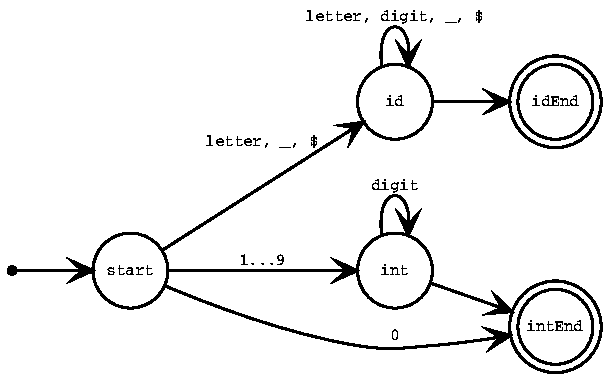
\includegraphics[scale=0.6]{{figures/figure02.01}.jpg}}
\end{center}

\begin{lstlisting}[language=Java]
    if (isLetter(ch) || ch == '_' || ch == '$') {
        buffer = new StringBuffer();
        while (isLetter(ch) || isDigit(ch) || ch == '_' || ch == '$'){
            buffer.append(ch);
            nextCh();
        }
        return new TokenInfo(IDENTIFIER, buffer.toString(), line);
    }
\end{lstlisting}
\end{frame}

\begin{frame}[fragile]
\pause

\begin{lstlisting}[language=Java]
    else if (ch == '0') {
        nextCh();
        return new TokenInfo(INT_LITERAL, "0", line);
    }
    else if (isDigit(ch)){
        buffer = new StringBuffer();
        while (isDigit(ch)) {
            buffer.append(ch);
            nextCh();
        }
        return new TokenInfo(INT_LITERAL, buffer.toString(), line);
    }
\end{lstlisting}
\end{frame}

\begin{frame}[fragile]
\pause

A state transition diagram for reserved words and the corresponding code
\begin{center}
\visible<2->{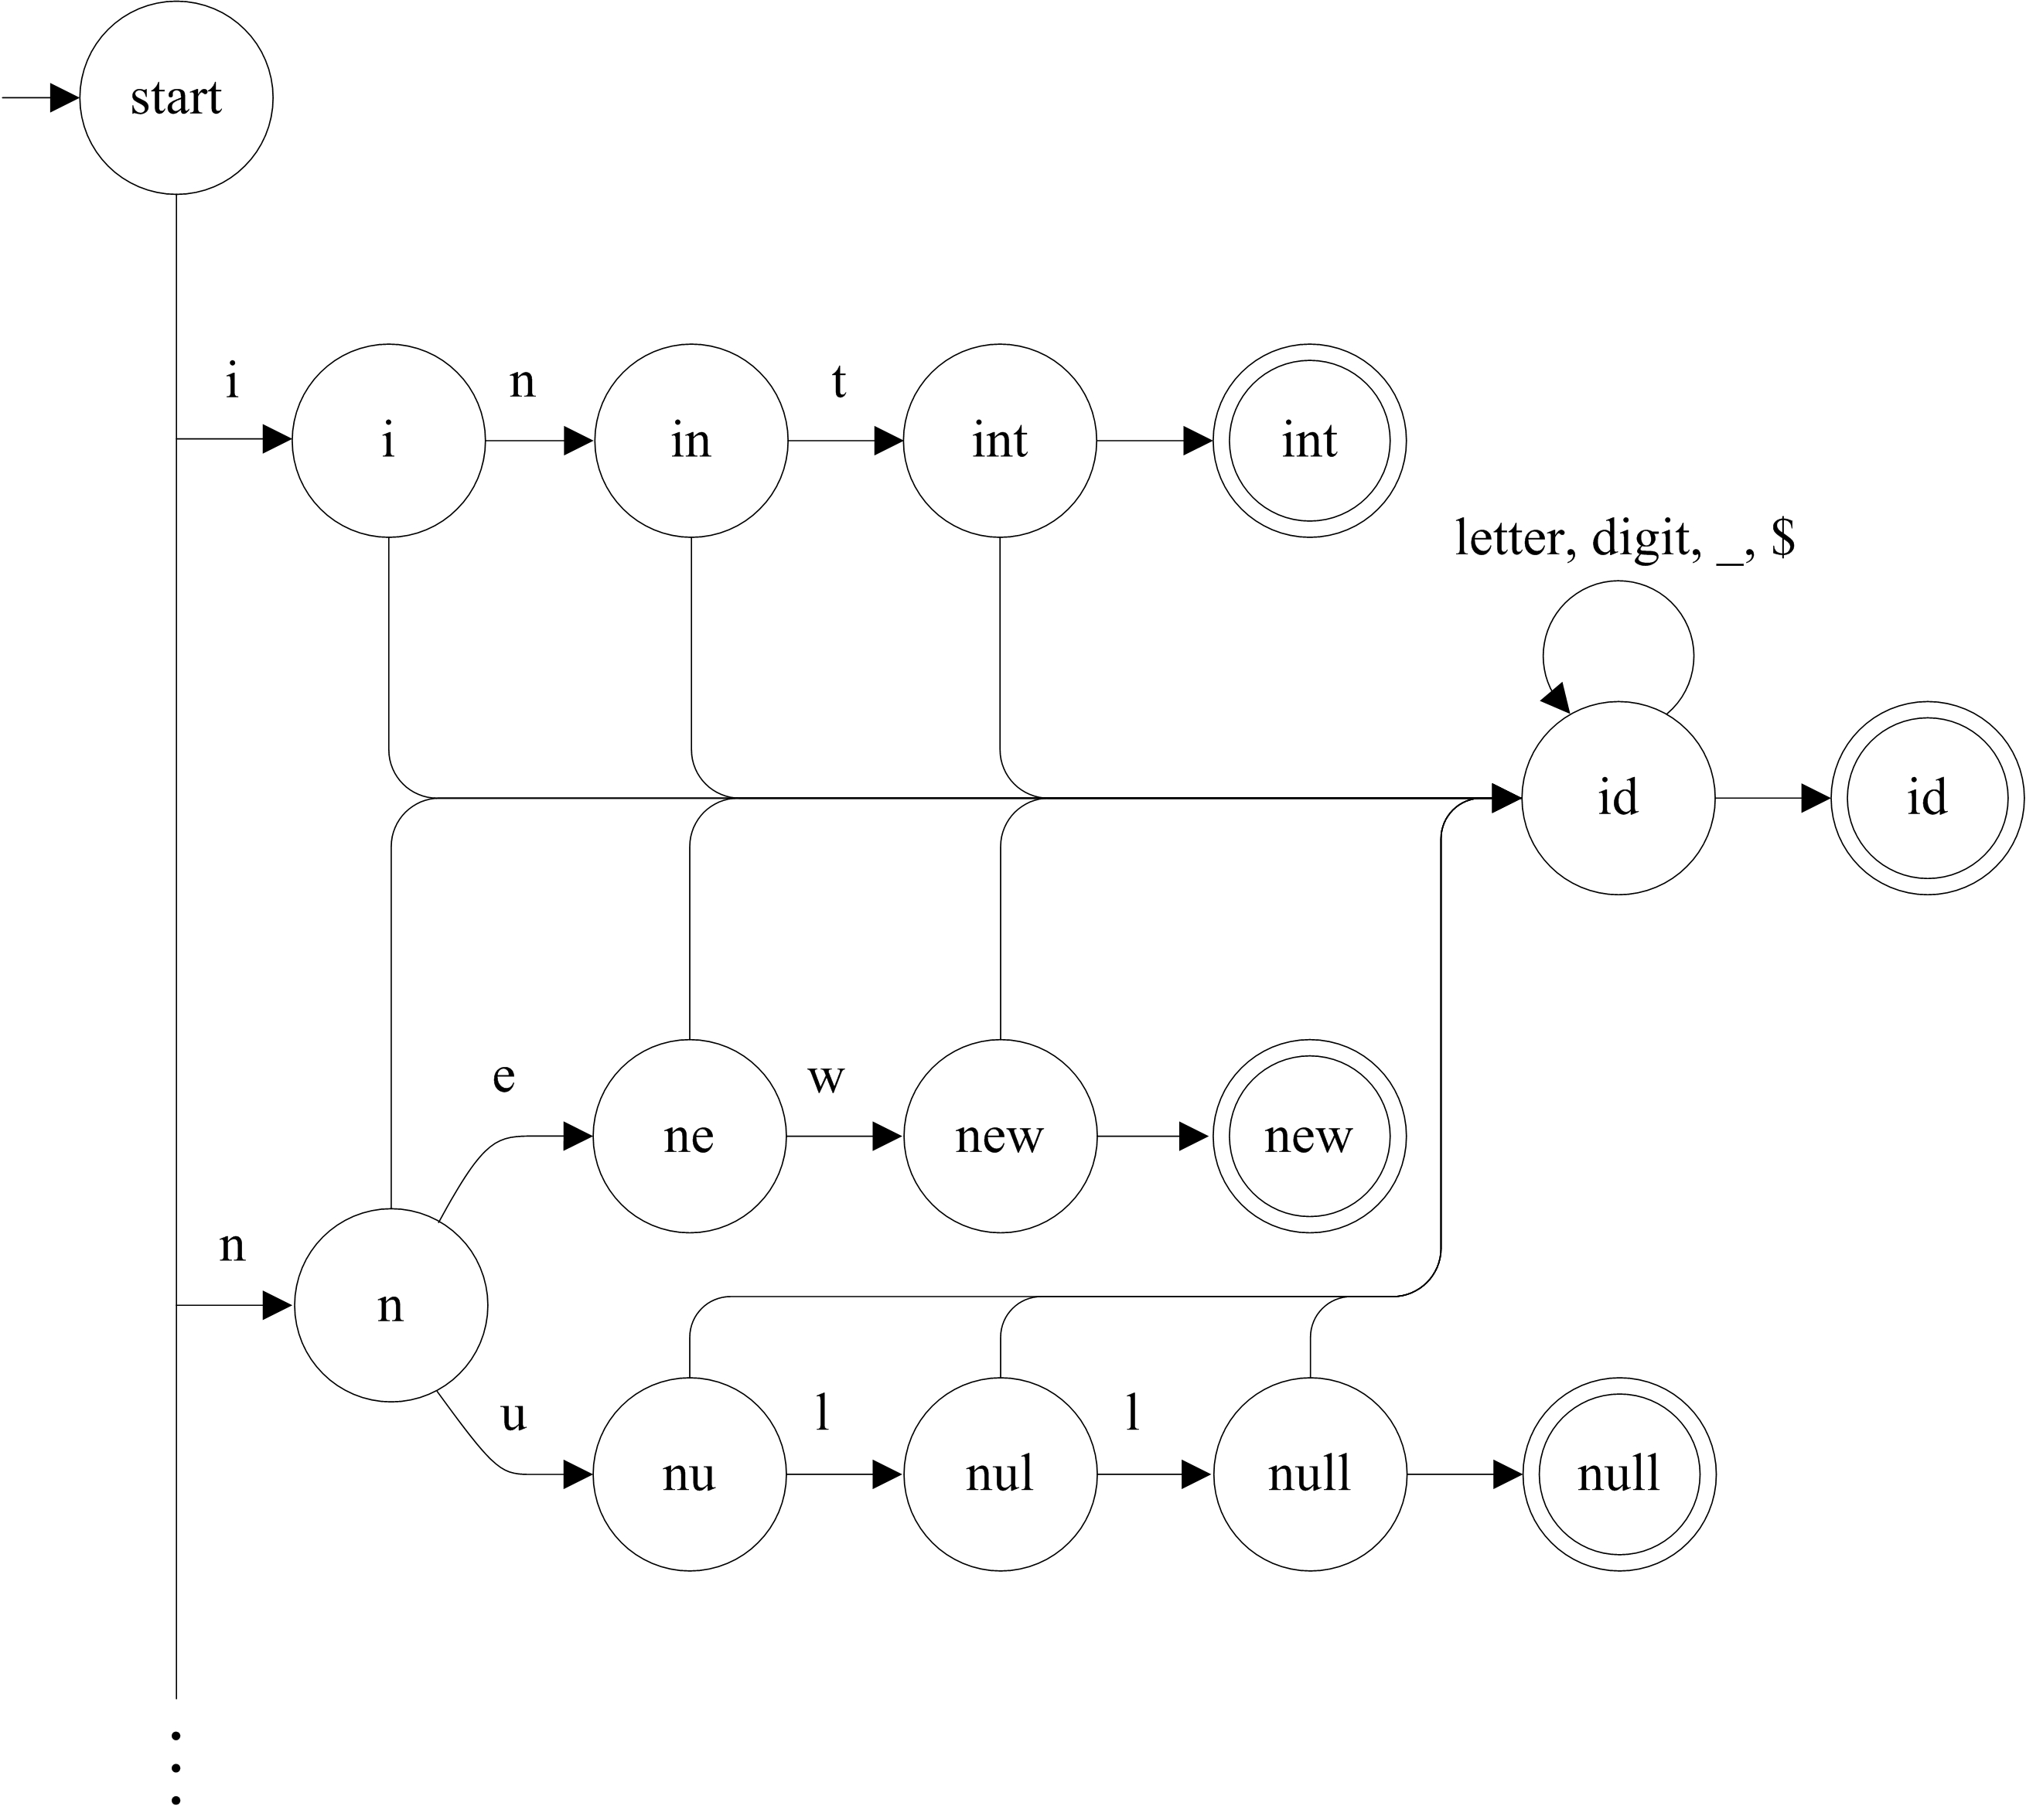
\includegraphics[scale=0.6]{{figures/figure02.02}.jpg}}
\end{center}
\end{frame}

\begin{frame}[fragile]
\pause

\begin{lstlisting}[language=Java]
...
else if (ch == 'n') {
    buffer.append(ch);
    nextCh();
    if (ch == 'e') {
        buffer.append(ch);
        nextCh();
            if (ch == 'w') {
            buffer.append(ch);
            nextCh();
            if (!isLetter(ch) && !isDigit(ch) && 
                     ch != '_' && ch !=  '$') {
                return new TokenInfo(NEW, line);
            }
        }
    }
    else if (ch == 'u') {
        buffer.append(ch);
        nextCh();
        if (ch == 'l') {
            buffer.append(ch);
            nextCh();
            if (ch == 'l') {
                buffer.append(ch);
                nextCh();
                if (!isLetter(ch) && !isDigit(ch) && 
                         ch != '_' && ch !=  '$') {
                    return new TokenInfo(NULL, line);
                }
            }
        }
    }
\end{lstlisting}
\end{frame}

\begin{frame}[fragile]
\pause

\begin{lstlisting}[language=Java]
    while (isLetter(ch) || isDigit(ch) || 
            ch == '_' || ch == '$') {
        buffer.append(ch);
        nextCh();
    }
    return new TokenInfo(IDENTIFIER, buffer.toString(), line);
}
else ...
\end{lstlisting}

\pause
\bigskip

A better approach for recognizing reserved words
\begin{center}
\visible<3->{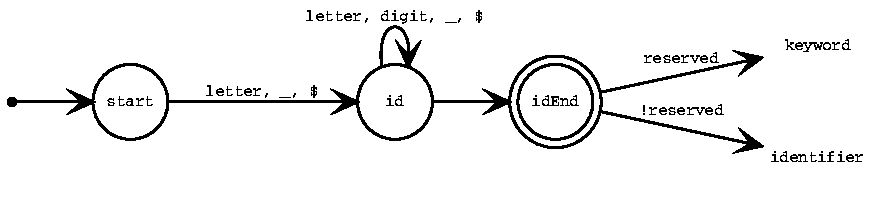
\includegraphics[scale=0.6]{{figures/figure02.03}.jpg}}
\end{center}
\end{frame}

\begin{frame}[fragile]
\pause

\begin{lstlisting}[language=Java]
    if (isLetter(ch) || ch == '_' || ch == '$') {
        buffer = new StringBuffer();
        while (isLetter(ch) || isDigit(ch) || 
               ch == '_' || ch == '$'){
            buffer.append(ch);
            nextCh();
        }
        String identifier = buffer.toString();                 
        if (reserved.containsKey(identifier)) {
            return new TokenInfo(reserved.get(identifier), line); 
        }
        else {                     
            return new TokenInfo(IDENTIFIER, identifier, line);                 
        }
    }
\end{lstlisting}

\pause
\bigskip

The above approach relies on a map (hash table), \lstinline{reserved}, mapping reserved identifiers to their representations:

\begin{lstlisting}[language=Java]
reserved = new Hashtable<String, Integer>();
reserved.put("abstract", ABSTRACT);  
reserved.put("boolean", BOOLEAN);         
reserved.put("char", CHAR);
...
reserved.put("while", WHILE);
\end{lstlisting}
\end{frame}

\begin{frame}[fragile]
\pause

A state transition diagram for separators and operators and the corresponding code
\begin{center}
\visible<2->{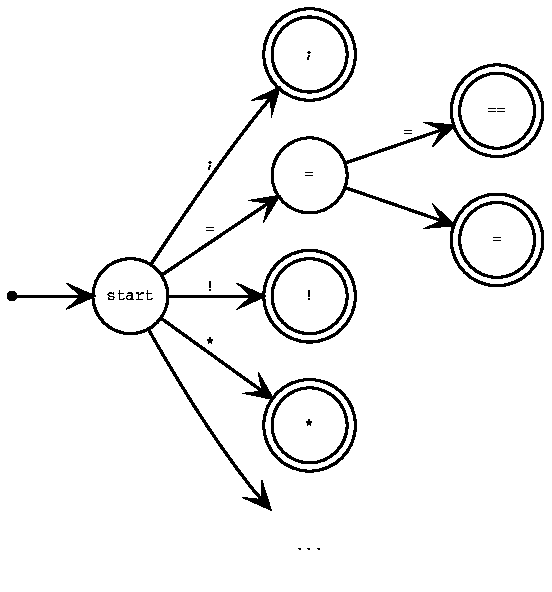
\includegraphics[scale=0.6]{{figures/figure02.04}.jpg}}
\end{center}
\end{frame}

\begin{frame}[fragile]
\pause

\begin{lstlisting}[language=Java]
switch (ch) {
...
case ';':
    nextCh();             
    return new TokenInfo(SEMI, line);         
case '=':             
    nextCh();             
    if (ch == '=') {                 
        nextCh();                 
        return new TokenInfo(EQUAL, line);             
    }             
    else {                 
        return new TokenInfo(ASSIGN, line);             
    }         
case '!':             
    nextCh();             
    return new TokenInfo(LNOT, line);         
case '*':             
    nextCh();             
    return new TokenInfo(STAR, line);
...
}
\end{lstlisting}
\end{frame}

\begin{frame}[fragile]
\pause

A state transition diagram for whitespace and the corresponding code
\begin{center}
\visible<2->{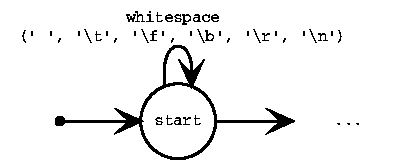
\includegraphics[scale=0.6]{{figures/figure02.05}.jpg}}
\end{center}

\begin{lstlisting}[language=Java]
while (isWhitespace(ch)) {                 
    nextCh();             
}
\end{lstlisting}
\end{frame}

\begin{frame}[fragile]
\pause

A state transition diagram for comments and the corresponding code
\begin{center}
\visible<2->{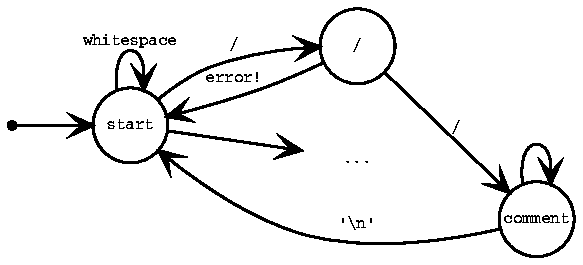
\includegraphics[scale=0.6]{{figures/figure02.06}.jpg}}
\end{center}
\end{frame}

\begin{frame}[fragile]
\pause

\begin{lstlisting}[language=Java]
boolean moreWhiteSpace = true;
while (moreWhiteSpace) {
    while (isWhitespace(ch)) {
        nextCh();
    }
    if (ch == '/') {
        nextCh();
        if (ch == '/') { 
            // CharReader maps all new lines to '\n'
            while (ch != '\n' && ch != EOFCH) {
                nextCh();
            }
        }
        else {
            reportScannerError("Operator / is not supported in j--.");
        }
    }
    else {
        moreWhiteSpace = false;
    }
}
\end{lstlisting}
\end{frame}

\section{Regular Expresssions}
\begin{frame}[fragile]
\pause

\end{frame}

\section{Finite State Automata}
\begin{frame}[fragile]
\pause

\end{frame}

\section{Non-deterministic (NFA) Versus Deterministic Finite State Automata (DFA)}
\begin{frame}[fragile]
\pause

\end{frame}

\section{Regular Expresssions to NFA}
\begin{frame}[fragile]
\pause

\end{frame}

\section{NFA to DFA}
\begin{frame}[fragile]
\pause

\end{frame}

\section{A Minimal DFA}
\begin{frame}[fragile]
\pause

\end{frame}

\section{JavaCC: a Tool for Generating Scanners}
\begin{frame}[fragile]
\pause

\end{frame}
\end{document}
